% generated by scripts/pkl_to_latex.py
% source PKL : thermal_v1_L6_Ne6_U10_t1_mode-uniform_tpall_t2all_tperpall_nmin2_solver-gcg_full_restarts10_iter300_kmax5_tol1em09_cut10_adaptive1_step5_clusteravg1_T0to0.289474_N12-f3dd7936eb54_knone_diag0.pkl
% C_GME for n = 4-6 from the tail rerun (*_tailrerun.pkl, hpc_tail/merge_thermal_tail.py)
% scan type  : Tscan
% state      : gs
% x-max cap  : 0.3 (cut at k_B T/t = 0.3, supervisor 4 Nov 2026)
% requires   : \usepackage{pgfplots} \pgfplotsset{compat=1.18}
% colours match the matplotlib PDF (tab10 cycle)
\definecolor{gmeC0}{HTML}{1F77B4}
\definecolor{gmeC1}{HTML}{FF7F0E}
\definecolor{gmeC2}{HTML}{2CA02C}
\definecolor{gmeC3}{HTML}{D62728}
\definecolor{gmeC4}{HTML}{9467BD}
\definecolor{gmeC5}{HTML}{8C564B}
\definecolor{gmeC6}{HTML}{E377C2}
\definecolor{gmeC7}{HTML}{17BECF}

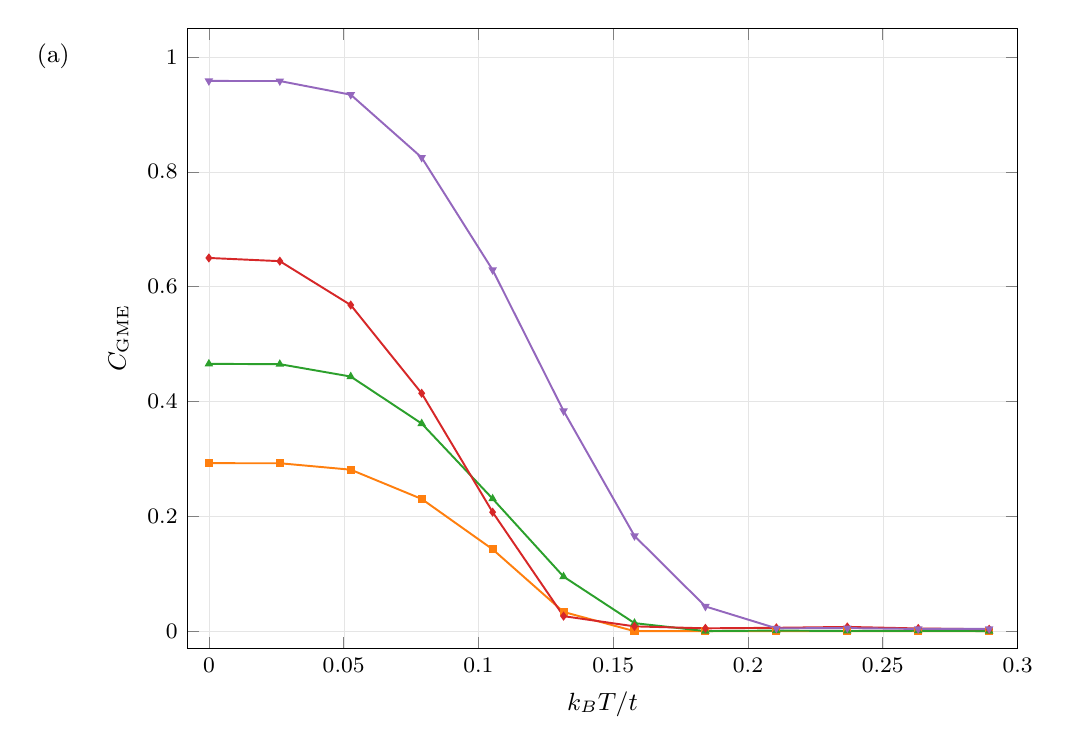
\begin{tikzpicture}
  \begin{axis}[
    width=\columnwidth,
    height=0.78\columnwidth,
    xlabel={$k_B T/t$},
    ylabel={$C_{\mathrm{GME}}$},
    grid=both,
    grid style={line width=.1pt, draw=gray!20},
    tick label style={font=\footnotesize\rmfamily, /pgf/number format/fixed},
    label style={font=\small\rmfamily},
    scaled ticks=false,
    legend style={font=\scriptsize\rmfamily, draw=gray!40, at={(0.5,1.03)}, anchor=south, /tikz/every even column/.append style={column sep=6pt}},
    legend cell align={left},
    legend columns=2,
    ymin=-0.03,
    ymax=1.05,
    xmin=-0.008,
    xmax=0.3,
    xtick={0,0.05,0.1,0.15,0.2,0.25,0.3},
    after end axis/.append code={\node[anchor=east, font=\small\rmfamily] at (axis description cs:-0.13,0.954) {(a)};},
  ]
    \addplot[color=gmeC1, mark=square*, mark size=1.1pt, line width=0.7pt] coordinates {
        (0,0.292503) (0.026316,0.29244) (0.052632,0.281207) (0.078947,0.230244)
        (0.105263,0.142587) (0.131579,0.033497) (0.157895,0.000003) (0.184211,0.000257)
        (0.210526,0.000012) (0.236842,0) (0.263158,0.000001) (0.289474,0.000003)
    };
    \addplot[color=gmeC2, mark=triangle*, mark size=1.1pt, line width=0.7pt] coordinates {
        (0,0.465509) (0.026316,0.464956) (0.052632,0.443399) (0.078947,0.361587)
        (0.105263,0.230658) (0.131579,0.095023) (0.157895,0.013998) (0.184211,0.000151)
        (0.210526,0.001028) (0.236842,0.000286) (0.263158,0.000721) (0.289474,0.000131)
    };
    \addplot[color=gmeC3, mark=diamond*, mark size=1.1pt, line width=0.7pt] coordinates {
        (0,0.649928) (0.026316,0.644347) (0.052632,0.567901) (0.078947,0.414213)
        (0.105263,0.207234) (0.131579,0.026156) (0.157895,0.008375) (0.184211,0.004952)
        (0.210526,0.005877) (0.236842,0.007407) (0.263158,0.00472) (0.289474,0.00334)
    };
    \addplot[color=gmeC4, mark=triangle*, mark size=1.1pt, mark options={rotate=180}, line width=0.7pt] coordinates {
        (0,0.958182) (0.026316,0.95803) (0.052632,0.934235) (0.078947,0.824809)
        (0.105263,0.62906) (0.131579,0.383589) (0.157895,0.165855) (0.184211,0.043035)
        (0.210526,0.004998) (0.236842,0.005354) (0.263158,0.003853) (0.289474,0.004091)
    };
  \end{axis}
\end{tikzpicture}
